\documentclass[conference]{IEEEtran}

\usepackage{graphicx}
\usepackage{url}

\newcommand{\todo}[1]{ \textbf{#1} }
\newcommand{\quotes}[1]{\textit{``#1''}}

% correct bad hyphenation here
\hyphenation{op-tical net-works semi-conduc-tor}


\begin{document}

\title{How do Scratch Users Name Variables and Functions? }

% author names and affiliations
% use a multiple column layout for up to three different
% affiliations
\author{\IEEEauthorblockN{Author1}
\IEEEauthorblockA{Uni1\\
Address1\\
Email: email1.com}
\and
\IEEEauthorblockN{Author2}
\IEEEauthorblockA{Uni2\\
	Address2\\
	Email: email2.com}}
% make the title area
\maketitle

% As a general rule, do not put math, special symbols or citations
% in the abstract
\begin{abstract}
The abstract goes here.
\end{abstract}

\IEEEpeerreviewmaketitle



\section{Introduction}
The naming of identifiers in the source code has been extensively studied (see, e.g., recent studies of this subject \cite{AmanASK15,AvidanF17,Beniamini,ButlerWYS10,HofmeisterSH17,LunguK13,ScannielloR13,TramontanaRS14}).
Still, the impact of the variable name choice on code readability and maintainability is controversial, as witnessed, e.g., by recent studies of Beniamini et al.~\cite{Beniamini} and Hofmeister et al.~\cite{HofmeisterSH17} reaching contradictory conclusions.
%Comprehension is linked to maintainability tasks and efficient performance of developers while performing them. \todo{AS says: we need either a citation to support this claim or rephrase} As one scientist once said \quotes{the code should be considered for human and less occasionally for a computer to execute}.\todo{AS asks: who has said this? This is a common adagio but I have no idea who is the author.}
%
Furthermore, computer science and programming education seem to focus on the programming concepts and the syntax of the languages as opposed to practices in naming variables and identifiers. 
Indeed, while ``meaningful variable names'' are advocated by some teachers~\cite{Kato2016} and practitioners~\cite{Rother} neither the ACM Curriculum Guidelines for Undergraduate Programs in Computer Science\footnote{\url{http://www.acm.org/education/CS2013-final-report.pdf}} nor the Curriculum Guidelines for Undergraduate Degree Programs in Software Engineering\footnote{\url{http://www.acm.org/binaries/content/assets/education/se2014.pdf}} discuss this topic.
In fact, one of the most common examples in many programming languages is the use of \quotes{foo} and \quotes{bar} naming for variables and functions. 
These two identifiers have meaningless names, and to some extent, they represent a refusal to name, suggesting the learner that the name is less important, or irrelevant, to the programming task. 

Recent studies have focused on the analysis of identifier naming in software code repositories. 
In this paper, we give attention to novice programmers with the Scratch visual language. 
When it comes to novice programmer and learners, it is more important for the software community to understand conceptions in naming that are prevalent. 
These users are the future developers, and at some point, they need to follow an implicit or explicit guideline of naming and collaborating in larger software repositories. 
To this end, we have analyzed 250,000 Scratch projects previously published by \cite{Aivaloglou2016HowKC}.
Scratch is a block-based visual language that was developed by MIT with the aim of helping young people learn the basic concepts of programming and collaboration.
Scratch has recently become very popular among school-age children and even in introduced as part of the school curriculum as a means to teach programming~\cite{SaezLopez}.
Analyzing Scratch programs will give researchers and software engineering community a perspective on naming from learners making their first step in programming and might turn to be the future programmers. In this paper we therefore aim at understanding \emph{how do Scratch users name variables and procedures? }

To answer this question we first replicate two studies from a recent paper by Beniamini et al.~\cite{Beniamini}.
We start by investigating the distribution of the lengths of variable and function names across Scratch projects. 
Next, we focus on popularity of single-letter names such as $i$ and $x$ as variable and function names.

To augment the previous study of Beniamini et al.~\cite{Beniamini} we focus on Scratch-specific features in naming identifiers.
In particular, we aim at understanding to what extent spaces within identifiers (e.g., variable \emph{max i}), digits as identifiers (e.g., variable 6) and parameters inserted the middle of the procedure name (\todo{Give an example}).
Those features are missing from the main-stream programming languages: if they will prove to be popular among the Scratch developers, one could advocate that they should be integrated in the main-stream programming languages as well.

\todo{More questions: analysis of the peak value of 5, what is the most recurrent name? Is it expected or justified?}
\todo{More questions: variable length based on category of the Scratch program: game animation, ....}
\todo{More questions: variable length in relation to Dr. Scratch CT}
 
\section{Background and motivation}
Naming identifiers in software code has been studied extensively in the past decades~\cite{AmanASK15,AnquetilL98,AvidanF17,Beniamini,ButlerWYS10,CaprileT00,HofmeisterSH17,LawrieMFB07,LunguK13,ScannielloR13,TakangGM96,TramontanaRS14}. 
In practice, identifiers constitute a major part of the source code: e.g., Dei{\ss}enb{\"o}ck and Pizka found that in Eclipse 3.0M7 which is tantamount to 2 MLoC, 33\% of the tokens and 72\% of characters correspond to identifiers~\cite{Deissenbock}. 
\todo{AS falling asleep, sorry}
For a human to read that code, it is crucial to understand what the identifier means, and then can deduce what the code does. 
With no surprise, several studies have confirmed the link between good identifier naming and code's readability and comprehension. 
The comprehension is not a target in its own; the true reason is that better comprehension lets the developers perform maintenance tasks more effectively and efficiently.
But what is a good naming approach? 
It is out of this paper's scope to explore the various recommendations of good identifier naming. 
However, it is worth to mention that there are different perspectives on what a good name is. 
Some researchers emphasize the usage of actual and complete words from a dictionary, or known abbreviations, which reflect the context of the program's purpose. 
Others argue that consistency in naming style is the most important. 
The usage of single-letter identifiers attracts much attention in research. 
For programmers, it is tempting to choose single-letter identifiers for quicker code writing that involves less mental load on the choice of a name. 
Additionally, single-letter named variables such as \quotes{i} or \quotes{j} have become almost a standard choice for index values when coding loops. 
Research has shown however that shorter identifier names are longer to comprehend, and the length of a variable should reflect its scope. 

Despite the agreement on the importance of identifier names, and efforts to introduce naming guidelines and additional tools to help the programmer choose better names, developers find giving appropriate names to identifiers as a difficult task. In the end, it is the decision of the individual writing the code, and many factors may contribute to that decision. One area to consider here is the computer science and in particular programming education. There seems to be a great focus on the programming concepts, while less to zero attention is given to beautifying the code. For example, the usage of the identifier names \quotes{foo} and \quotes{bar} is prevalent in code examples. These names have no real meaning, and the student cannot link them to what the code does.  

We are inspired by the work done by \todo{ref} where they explored the single-letter naming for multiple software repositories from different programming languages. It is important for the software community to understand the patterns in which software developers apply naming to identifiers. We argue that this understanding can improve the quality of the guidelines and introduce research-supported tools that meet the needs of the programmers. For this sake, we believe it is even more important to focus on the novice programmers, students, and learners. For these future developers, the usage of a particular naming pattern in this level forms a (mis)conception that could move along with them to other programming languages and future careers. The work was done by \todo{add ref} excludes the visual languages which have recently become a favorable choice for elementary and high schools as an introduction to programming, for example, Scratch and Alice. These block-based languages allow the user to create and assign their identifiers for variables and blocks. By studying these identifiers, we can understand better how novice programmers apply standard and language-specific naming, and how it compares to other textual based languages previously explored in the literature. 

\section{Relevant Scratch Concepts}
\label{sec:scratch}
This paper is by no means an introduction into Scratch programming, we refer the reader to \cite{brennan_creative_2014} for an extensive overview. To make this paper self-contained, however, we explain a number of relevant concepts in this section. 

Scratch is a block-based programming language aimed at children, developed by MIT. Scratch can be used to create games and interactive animations, and is available both as a stand-alone application and as a web application. Figure \ref{fig:ui} shows the Scratch user interface in the Chrome browser.

\subsection{Sprites}
Scratch code is organized by `sprites': two-dimensional pictures each having their own associated code. Scratch allows users to bring their sprites to life in various ways, for example by moving them in the plane, having them say or think words or sentences via text balloons, but also by having them make sounds, grow, shrink and switch costumes. The Scratch program in Figure \ref{fig:ui}\footnote{\url{https://scratch.mit.edu/projects/97086781/}} consists of one sprite, the cat, which is Scratch's default sprite and logo. The code in the sprite will cause the cat to jump up, say ``hello'', and come back down, when the green flag is clicked, and to make the `meow' sound when the space bar is pressed.

\begin{figure}
  \begin{center}
  \includegraphics[width=\columnwidth]{fig/ui.png}
  \caption{The Scratch user interface consisting of the `cat' sprite on the left, the toolbox with available blocks in the category `motion' in the middle and the code associated with the sprite on the right. The upper right corner shows the actual location of the sprite.}
  \label{fig:ui}
  \end{center}
\end{figure} 

\subsection{Events}
Scratch is \emph{event-driven}: all motions, sounds and changes in the looks of sprites are initiated by events. The canonical event is the `when Green Flag clicked', activated by clicking the green flag at the top of the user interface. In addition to the green flag, there are a number of other events possible, including key presses, mouse clicks and input from a computer's microphone or webcam. In the Scratch code in Figure \ref{fig:ui} there are two events: `when Green Flag clicked' and `when space key pressed'

\subsection{Scripts}
Source code within sprites is organized in scripts: a script always starts with an event, followed by a number of blocks. The Scratch code in Figure \ref{fig:ui} has two distinct scripts, one started by clicking on the green flag and one by pressing the space bar. It is possible for a single sprite to have multiple scripts initiated by the same event. In that case, all scripts will be executed simultaneously. 

\subsection{Remixing}
Scratch programs can be shared by their creators in the global Scratch repository\footnote{\url{https://scratch.mit.edu/explore/projects/all/}}. Shared Scratch programs can be `remixed' by other Scratch users, which means that a copy of this program is placed in the user's own project collection, and can be then further changed. The `remix tree' of projects is public, so users can track which users remix their programs, a bit similar forking in GitHub. Contrary to forking however, changes upstream cannot be integrated back into the original project. Because Scratch users can remix each others programs, maintainability of programs is important. A given Scratch program can be read and adapted by many children, there are projects on the Scratch home page which are remixed hundreds of times. \todo{maybe this part about importance should be move somewhere else? this section might be skipped.}

\subsection{Variables}
Like most textual languages, Scratch users can use variables. Variables are untyped, but have to be `declared' through the Scratch user interface, shown in Figure \ref{fig:ui-vars}. This figure also shows that, contrary to most programming languages, variable names in Scratch may contain spaces.

\begin{figure}
  \begin{center}
  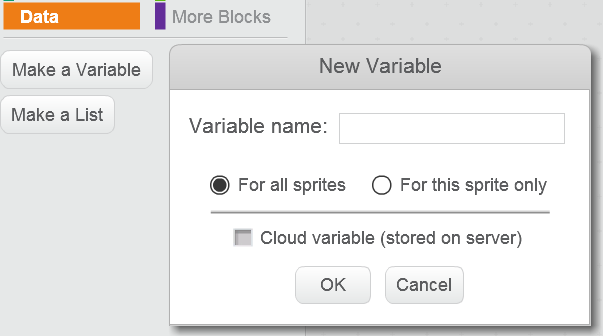
\includegraphics[width=\columnwidth]{fig/ui-vars.png}
  \caption{The Scratch user interface to create a variable}
  \label{fig:ui-vars}
  \end{center}
\end{figure} 

\subsection{Procedures}
Scratch also allows users to create their own blocks, called procedures. They can have input parameters, and labels in between them. Functions are created with an interface similar to the one to create variables. Figure \ref{fig:functions} shows the definition and invocation of a procedure.

\begin{figure}
  \begin{center}
  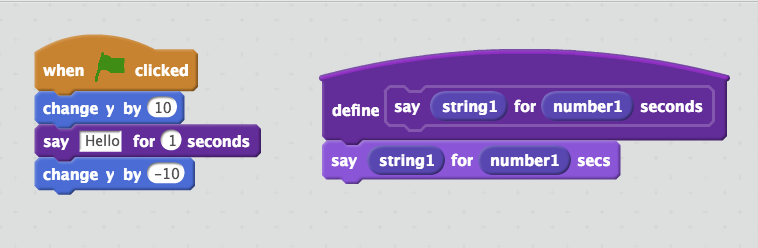
\includegraphics[width=\columnwidth]{fig/functions.png}
  \caption{Scratch code to define and invoke a procedure}
  \label{fig:functions}
  \end{center}
\end{figure} 


\section{Research design and dataset}
\subsection{Overall design}
As our goal is to compare the naming practices among the Scratch-developers with those of the developers in the mainstream programming languages we start by partially replicating the recent work of Beniamini et al. on the use of single-letter variables in Java, C, PHP, Perl and JavaScript~\cite{Beniamini}. 
In terms of the classification of Shull et al.~\cite{Shull2008} we perform a dependent replication of the studies summarized in Figures 1 and 2 of the original work by Beniamini et al.~\cite{Beniamini}.  
 Inherently, the programming language is the only factor we vary when compared to the original study.
However, as Scratch programs are not available on GitHub that has been used in the study of Beniamini et al., \todo{Felienne, is this true?} we also had to change the source of the data.

Next, we perform a conceptual replication of the study of the single-letter variable types of Beniamini et al.~\cite{Beniamini}. 
While the original study has conducted a survey to understand the type-related user perceptions (``what type would you consider for a variable called ...?'') we focus on the types as defined in the program. 
\todo{Felienne, Alaaeddin, can we explain why would we prefer to analyze types as opposed to the survey? Time?}

Finally, to augment this study we also investigate the ways Scratch developers can benefit from Scratch-specific naming practices such as spaces in variable names, digits as variables and use of textual labels in between parameters.

\subsection{Dataset}
For this paper we use the dataset created by Aivaloglou and Hermans~\cite{Aivaloglou2016HowKC}, consisting of 250.000 Scratch projects scraped from the Scratch website in March 2016. From this dataset, we have selected the projects that use variables or functions, together this are 73.473 projects (29\%) of Aivaloglou and Hermans's original dataset. Variable use is more common that procedure use. In total 69.045 projects (27.6\%) use variables, while 17.605 use procedures (7.0\%). We used Python to process the original dataset and generate the graphs in this paper. The code we used is available at \url{https://github.com/Felienne/ScratchVars}.

\subsection{Data analysis}
\label{sec:da}
To augment the visual comparison of the variable name data derived from Scratch as well as the programming languages considered by Beniamini et al.~\cite{Beniamini}, we conduct statistical analysis. 

Understanding differences in variable name lengths requires comparison of multiple distributions, traditionally performed as a two-step process consisting of (1) testing a global null hypothesis, that can be intuitively formulated as ``all distributions are the same'', using ANOVA or its non-parametric counterpart, the Kruskal-Wallis test, and (2) performing multiple pairwise comparisons of different distributions, testing specific subhypotheses such as ``distributions 2 and 4 are the same''. 
However, it has been observed that such a two-step approach can result in inconsistencies when either the global null hypothesis is rejected but none of the pairwise subhypotheses is rejected or vice versa~\cite{Gabriel}. 
Moreover, it has been suggested that the Wilcoxon-Mann-Whitney test, commonly used for subhypothesis testing, is not robust to unequal population variances, especially in the unequal sample size case~\cite{Zimmerman:Zumbo}
Therefore, one-step approaches have been sought.
We opt for one such approach, the $\widetilde{\mathbf{T}}$-procedure of Konietschke et al.~\cite{Konietschke:Hothorn:Brunner}. 
This procedure is robust against unequal population variances, respects transitivity, and has been successfully applied in empirical software engineering~\cite{VasilescuSGM14,VasilescuCS14,YuWYW16}.
In particular, we use the Tukey (all-pairs) contrasts to compare all distributions pairwise.

Furthermore, to understand differences and similarities between the distributions of single-letter variable names in different languages we represent each programming language as a 26-dimensional vector with the dimensions corresponding to `a', ..., `z', and apply hierarchical clustering. \todo{why hierarchical?}

\todo{where does this belong? and is this still true?}
Unless indicated otherwise, all graphs show the number of projects a certain type of variable is used in, rather then the number of occurrences of the variable. Some projects access and update variables hundreds of times, so we felt that counting use would skew the graphs towards bigger programs.
\todo{maybe this paragraph fits with dataset more than with results? Not sure.}

 \section{Results}
This section presents an overview of our analysis of variable and function name use in our previously published Scratch dataset~\cite{Aivaloglou2016HowKC}. 

\subsection{Variable name length}
The original study of Beniamini et al.~\cite{Beniamini} has concluded that the single-letter variable names ``are approximately as common as other short lengths except in PHP'' and that  ``in C, Java, and Perl they make up 9–20\% of the names.'' 
Figure~\ref{fig:distribution_of_lengths} shows the distribution of lengths in the Scratch corpus. 
Closer look at the data reveals that the single-letter variables constitute ca. 4.9\% of all the names used in the program, i.e., less than the 9-20\% observed by Beniamini et al.

\begin{figure}[tb]
	\begin{center}
		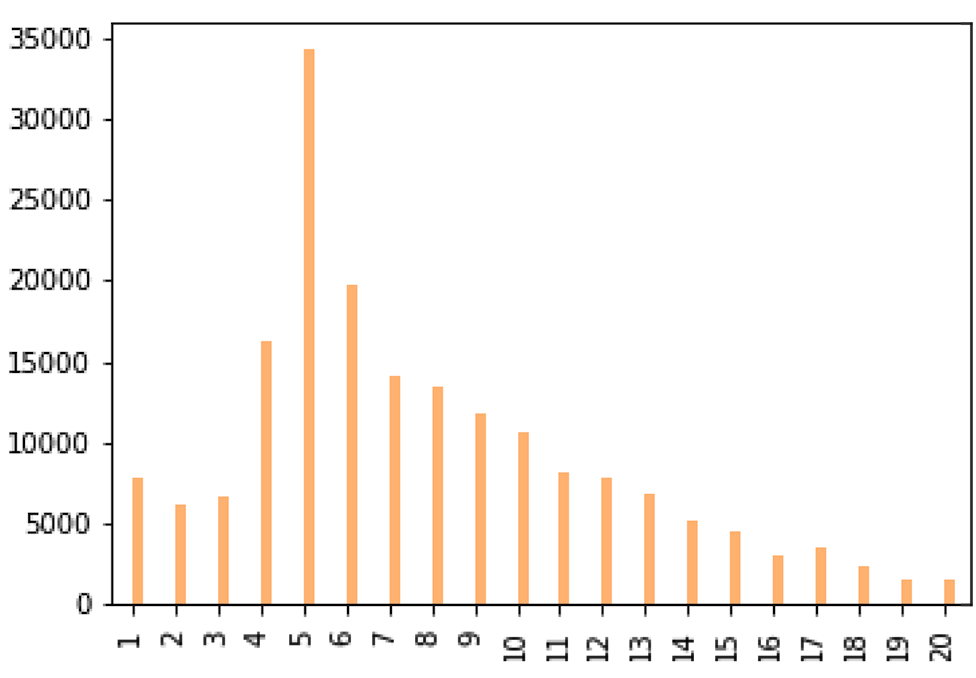
\includegraphics[width=\columnwidth]{fig/distribution_of_lengths}
		\caption{Frequency of  variables with names of different lengths}
		\label{fig:distribution_of_lengths}
	\end{center}
\end{figure} 
\todo{still need to add the 20+ bucket if we want to have that}

Since single-letter variables seem to be less common in Scratch than in the mainstream programming languages we wonder whether overall the variable names in Scratch tend to be longer than in other programming languages.
To this end we apply the $\widetilde{\mathbf{T}}$-procedure described in Section~\ref{sec:da}. 
Statistical analysis reveals that indeed, variable names in Scratch tend to be longer than in the mainstream languages.
Moreover, variable names in Java tend to be longer than those in PHP, variable names in  PHP than those in C, variable names in C than those in JavaScript and finally variable names in JavaScript longer than those in Perl. 
In all cases $p$-values have been too small to be computed precisely.

We conclude that single-letter variable names are less common in Scratch than in other programming languages and that overall Scratch variables have longer names than variables in other programming languages.

\subsection{Single-letter variable names}

 The authors have made the following observations about single-letter variable names:
\begin{enumerate}
\item The most commonly occurring single-letter variable name is $i$. The authors attribute this to $i$ being commonly used as a loop counter. Since Scratch supports loops, we expect $i$ to be commonly used in Scratch as well. \label{single-letter-vars:i}
\item Apart from the popularity of $i$ the distribution is language-dependent. Since Scratch is quite different from the mainstream programming languages considered by Beniamini et al., we expect the distribution of the single-letter variable names to be different from the distributions in these languages. 
Hence, we expect the \emph{similarity} between Scratch and the languages considered by Beniamini et al. to be lower than the \emph{similarity} between the languages considered by Beniamini et al. \todo{Felienne, Alaaeddin: do we agree with this hypothesis?} \label{single-letter-vars:similarity}
\item Finally, they observe that the lower case letters are used more frequently than the upper case letters. Since this is also the case for regular text in most natural languages as well, we expect the Scratch programs to follow the same pattern. \label{single-letter-vars:upercase:lowercase}
\end{enumerate}

Figure \ref{fig:one_letter_occurrence} shows the distribution of variables of one letter in the corpus. 
Inspecting the data we observe that similarly to the previous study $i$ is one of the most commonly occurring variables. 
Hence, we conclude that Observation~\ref{single-letter-vars:i} above also holds for Scratch.
\todo{Felienne, Alaaeddin: For Observation~\ref{single-letter-vars:similarity} I would like to hear your opinion on the hypothesis first, and then we need to separate upper case and lower case since similarity will depend on this separation. For Observation~\ref{single-letter-vars:upercase:lowercase} we clearly need to separate upper and lower case.}

Furthermore, we observe that $x$ and $y$ are extremely popular in Scratch.
This can be explained by observing that $x$ and $y$ are default variables in Scratch, representing the position of \todo{Felienne, of sprite? of what else?}

\todo{Felienne, Alaaeddin: any other observations?}

\todo{Felienne, please remove the ``project id'' legend as it is confusing}

\begin{figure}[h]
	\begin{center}
		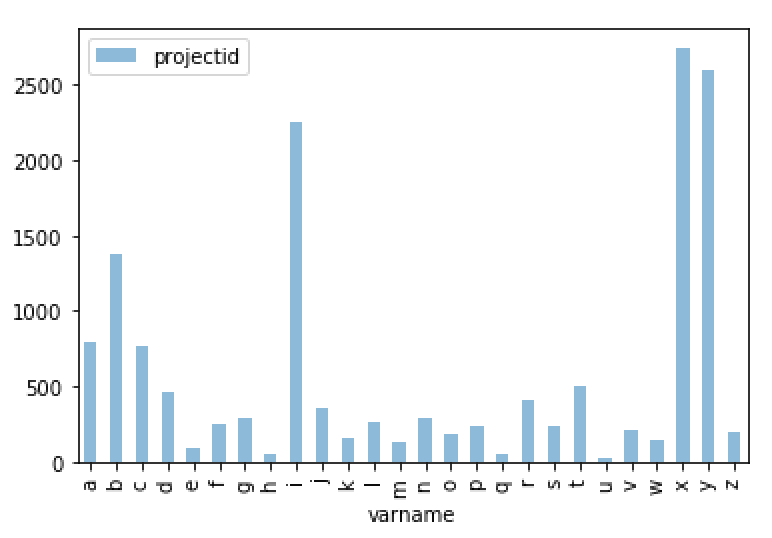
\includegraphics[width=\columnwidth]{fig/one_letter_occurrence}
		\caption{Number of projects using variables of each of the one letter variables}
		\label{fig:one_letter_occurrence}
	\end{center}
\end{figure} 

Going beyond the study of Beniamini Figure \ref{fig:one_letter_occurrence_functions} shows the distribution of \emph{functions} of one letter in the corpus.
By inspecting this figure we observe \todo{Alaaeddin, please continue here.}

\begin{figure}[h]
	\begin{center}
		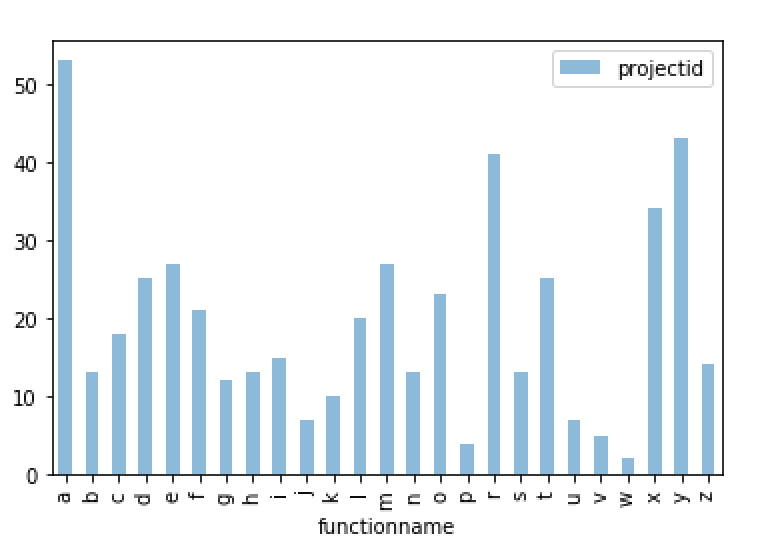
\includegraphics[width=\columnwidth]{fig/one_letter_occurrence_functions}
		\caption{Total occurrence of functions of one letter}
		\label{fig:one_letter_occurrence_functions}
	\end{center}
\end{figure} 

\subsection{Types}
Beniamini et al.~\cite{Beniamini} also explored the types of one letter variables, by performing a questionnaire among \todo{summary of study here}.

This gave us the idea to also explore types of one letter variables in the context of our dataset. While Scratch variables have no types, we can deduce their use from our dataset, by exploring what assignments are made to variables and deducing the types from those. For example, the two variables in Figure \ref{fig:types} represent a string and an integer respectively. With this process we can compare our results to the types of Beniamini et al.~\cite{Beniamini}. 
Figure \ref{fig:one_letter_type} shows the distribution of variables of one letter in the corpus.

\begin{figure}
	\begin{center}
		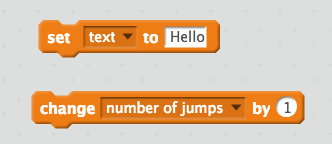
\includegraphics[width=5cm]{fig/types}
		\caption{Two variables, one of type string and one of type integer}
		\label{fig:types}
	\end{center}
\end{figure} 

\todo{here we need to write some reflection on the results. Alaaeddin....? :-) Comparing the results with the other languages and between functions and variables.}

\begin{figure}
	\begin{center}
		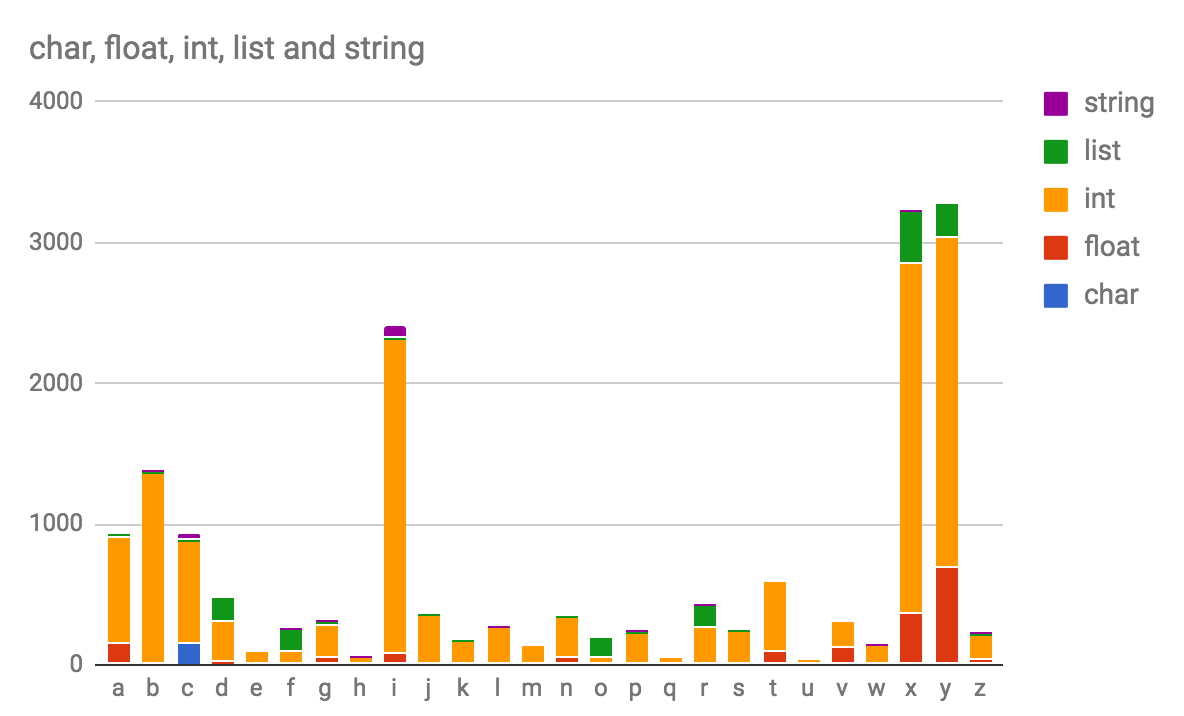
\includegraphics[width=\columnwidth]{fig/one_letter_type}
		\caption{Inferred types for variables of one letter}
		\label{fig:one_letter_type}
	\end{center}
\end{figure} 


\section{Scratch specific constructs}



\subsection{Use of spaces in variable names}

Contrary to most textual programming languages, Scratch allows users to use spaces in variable names. This is quite commonly used, about 30.000 projects use one or more variables with a space in it, versus 60.000 that use only space-free variable names. Figure \ref{fig:number_of_spaces} shows the distribution of spaces in variable names. We have found that many introductory Scratch programming materials demonstrate the use of space free variables, and that children---and adults---that already have programming experience deem the use of spaces in variables as non-natural, even though arguable `number of apples' is more natural that `nApples'.

\begin{figure}
	\begin{center}
		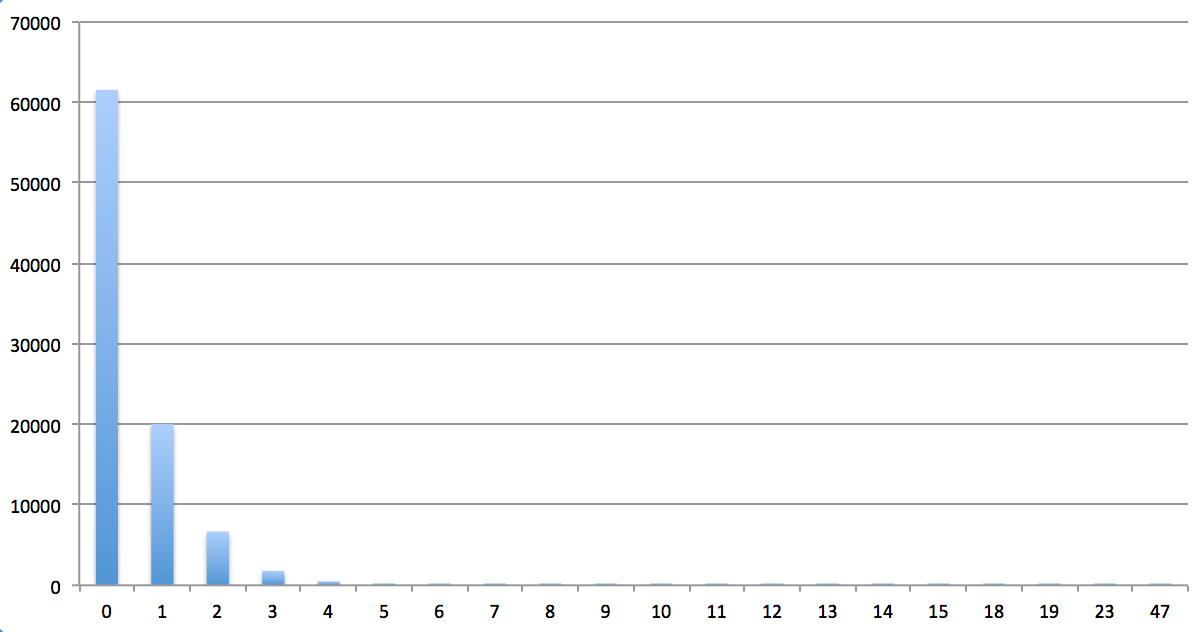
\includegraphics[width=\columnwidth]{fig/number_of_spaces}
		\caption{Number of spaces in variable names}
		\label{fig:number_of_spaces}
	\end{center}
\end{figure} 

\subsection{Use of numeric variable names}
In addition to spaces in variable names, Scratch even allows the use of numbers and even floating point numbers as variables. We found 718 projects with integer variable names and 19 with floating point names. While their use is rare, we manually examined some projects and numbers are used in interesting and clever ways.

\begin{figure}
	\begin{center}
		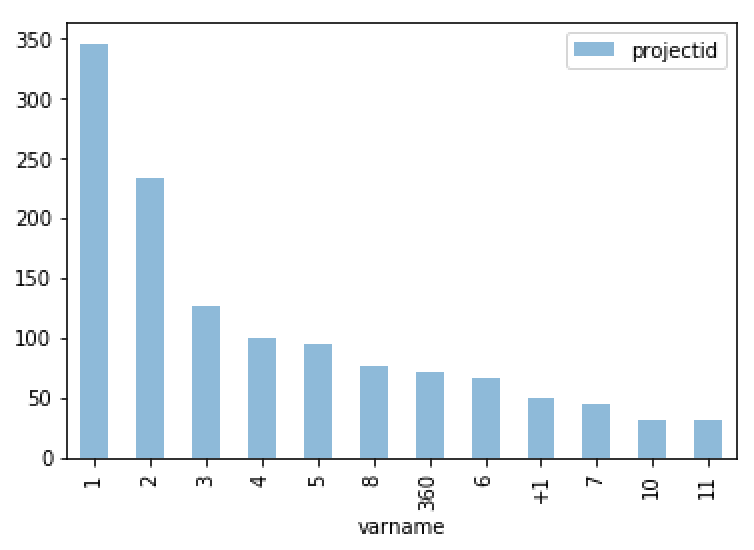
\includegraphics[width=\columnwidth]{fig/numeric}
		\caption{Number of projects using the most popular numeric variables}
		\label{fig:numeric}
	\end{center}
\end{figure} 

\todo{it seems these things are mainly used as constants. We could explore the dataset a bit to find out!}

\todo{here we can show the tic tac toe example}

\subsection{Use of textual labels in between parameters}

As can be seen in Figure \ref{fig:functions}, Scratch allows users to insert textual labels in between parameters in order to make functions more readable. Scratch built-in blocks use a similar syntax, for example in the ``say ... for ... seconds" block. In total 4415 projects use textual labels, so their use if not that common. We do however find some interesting patterns. Figure \ref{fig:labels} shows the most commonly used labels. Here we see some patterns common in textual languages, like the use of labels for the names of the parameters `x:' and `y:'. Furthermore we see the use of `)', which could come from textual languages too. Finally the use of the space is interesting, since Scratch already leaves some room between the parameters, also when a space is not used. The use of space as a separator could indicate that Scratch users feel room between variables is currently too small.

\begin{figure}
	\begin{center}
		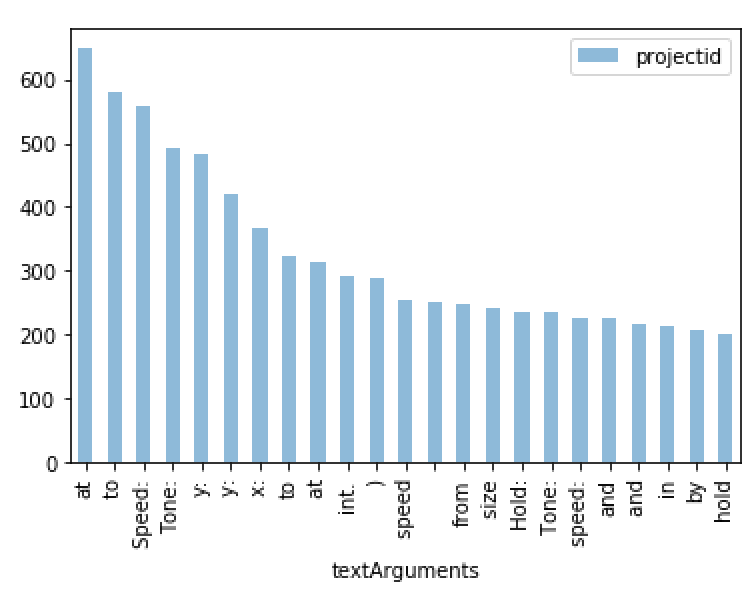
\includegraphics[width=\columnwidth]{fig/labels}
		\caption{Number of projects using the most popular numeric variables}
		\label{fig:labels}
	\end{center}
\end{figure} 



 \section{Discussion}


\section{Conclusion}
The conclusion goes here.




% conference papers do not normally have an appendix


% use section* for acknowledgment
\section*{Acknowledgment}


The authors would like to thank...





% trigger a \newpage just before the given reference
% number - used to balance the columns on the last page
% adjust value as needed - may need to be readjusted if
% the document is modified later
%\IEEEtriggeratref{8}
% The "triggered" command can be changed if desired:
%\IEEEtriggercmd{\enlargethispage{-5in}}

% references section

% can use a bibliography generated by BibTeX as a .bbl file
% BibTeX documentation can be easily obtained at:
% http://mirror.ctan.org/biblio/bibtex/contrib/doc/
% The IEEEtran BibTeX style support page is at:
% http://www.michaelshell.org/tex/ieeetran/bibtex/
\bibliographystyle{IEEEtran}
% argument is your BibTeX string definitions and bibliography database(s)
\bibliography{paper}
%
% <OR> manually copy in the resultant .bbl file
% set second argument of \begin to the number of references
% (used to reserve space for the reference number labels box)

% that's all folks
\end{document}


